% IEEE standard conference template; to be used with:
%   spconf.sty  - LaTeX style file, and
%   IEEEbib.bst - IEEE bibliography style file.
% --------------------------------------------------------------------------

\documentclass[letterpaper]{article}

\usepackage{spconf,amsmath,amssymb,graphicx,hyperref,subcaption,changes}
\usepackage{algorithm,algpseudocode} %algorithmicx

% |X|
\newcommand{\abs}[1]{\left| #1 \right|}
%keywords
\newcommand{\kif}[0]{\textbf{if}\hspace{1mm}}
\newcommand{\kthen}[0]{\textbf{then}\hspace{1mm}}
\newcommand{\kand}[0]{\hspace{1mm}\textbf{and}\hspace{1mm}}
% bold paragraph titles
\newcommand{\mypar}[1]{{\bf #1.}}
\definechangesauthor[name={Roman}, color=orange]{R}
% Title.
% ------
%% TODO
\title{Something with connected components}
%
% Single address.
% ---------------
\name{Giovanni Balduzzi, Michael Bernasconi, Lea Fritschi, Roman Haag}
\address{Department of Computer Science\\ ETH Z\"urich\\Z\"urich, Switzerland}

% For example:
% ------------
%\address{School\\
%		 Department\\
%		 Address}
%
% Two addresses (uncomment and modify for two-address case).
% ----------------------------------------------------------
%\twoauthors
%  {A. Author-one, B. Author-two\sthanks{Thanks to XYZ agency for funding.}}
%		 {School A-B\\
%		 Department A-B\\
%		 Address A-B}
%  {C. Author-three, D. Author-four\sthanks{The fourth author performed the work
%		 while at ...}}
%		 {School C-D\\
%		 Department C-D\\
%		 Address C-D}
%

\begin{document}
%\ninept
%
\maketitle

%The hard page limit is 6 pages in this style. Do not reduce font size
%or use other tricks to squeeze. This pdf is formatted in the American letter format, so the spacing may look a bit strange when printed out.

\begin{abstract}
We present an improved parallel implementation of a tree based connected components algorithm originally
introduced in 1984 by U. Vishkin. To improve the algorithm's performance the graph's edges are
distributed across multiple cores. Each process computes in a lock-free manner a local forest representing the different
connected components. The resulting forests are then combined using a reduction. A comparison of our
algorithm against a communication avoiding algorithm recently developed at ETH, on a set of large graphs
($5\times10^8$ Edges with up to $2\times10^7$ Vertices), is presented. Results where our algorithm uses a
mixture of both MPI and OMP are also shown.
\end{abstract}

\section{Introduction}\label{sec:intro}



\mypar {Motivation}
\replaced{Problems in computer science are often modeled as graphs.}{In computer science problems often get model as graphs and} Therefore, graph algorithms are ubiquitous. One of these graph problems is \deleted{the task of} finding \deleted{the} connected components in a graph. It is a well understood problem in graph theory with a variety of applicable domains. Computer vision tasks, such as pattern recognition and image segmentation \cite{683775} can make use of connected components \cite{Wilson:2006:RCV:1166253.1166292}. Other fields are medical imaging \cite{UDUPA1990355} and image processing \cite{Ambrosio2001}. \replaced{The related problem of strongly connected components will not be discussed in this paper}{We will not discuss the related problem of strongly connected components}.

\deleted{As already mentioned this problem is well-studied both sequentially and in parallel.} The first sequential algorithm \added{to solve the connected components problem} goes back to \cite{Hopcroft}. \deleted{A few} Parallel approaches \deleted{would be} \added{were presented in }\cite{MANOHAR1989133} \added{and} \cite{Han:1990:EFP:79147.214077} \added{.} \deleted{and} Recently \cite{comm_avoiding} \added{was published,} where \deleted{they used} a communication-avoiding approach \added{was discussed}. A communication-avoiding algorithm uses asymptotically less communication. By doing so \cite{comm_avoiding} sacrifices some \added{computational} efficiency \deleted{in the computation} as the root node does most of the work. \replaced{In this paper we present an algorithm which distributes the work while still avoiding as much communication as possible.}{We wanted to improve on this by also introducing a distributed computation based on hooking \cite{article} and ignoring the communication part.} \deleted[remark=this does not belong in the motivation]{In a additional step we distributed the list of edges evenly among different MPI proccesses. This allows us to outperform the communication avoiding approach especially on denser graphs. Our approach perfroms significantly worse on a small amount of nodes (n$\leq$ 5) but as we increase the total number of cores the benefits of our algorithms starts to show.}




\mypar{Connected components}
%Precisely define sorting problem you consider.
%\mypar{Sorting algorithms}
%Explain the algorithm you use including their costs.
%
%As an aside, don't talk about "the complexity of the algorithm.'' It's incorrect,
%problems have a complexity, not algorithms.

For an undirected graph $G=(V,E)$, the connected components are the ensemble
of connected subgraphs, where connected means that for any two vertices there exists a path along
the edges connecting them.
A straightforward algorithm to find the connected components is to perform either
a breath or depth first search starting from a random vertex in $V$,
and give the same label to all vertices reached. The search is then repeated, starting from an
unlabeled vertex.
This has a cost in terms of memory accesses of $\Theta(\abs{E} + \abs{V})$, which turns out
to be optimal \cite{Hopcroft}.

\section{Proposed Algorithm}\label{sec:yourmethod}
%Now comes the ``beef'' of the report, where you explain what you
%did. Again, organize it in paragraphs with titles. As in every section
%you start with a very brief overview of the section.
%
%In this section, structure is very important so one can follow the technical content.
%
%Mention and cite any external resources that you used including libraries or other code.


Unfortunately this algorithm does not parallelize in a straightforward
way. Instead we first implemented
an algorithm proposed by Uzi Vishkin \cite{PCompArticle} and later described in a class by Pavel
Tvrdik \cite{PCompClass}. This algorithm casts the problem in terms of the generation of a
forest, where the vertices of the same connected component belong to the same tree, and its root
can be used as the representative.\\
We define a star as a tree of height one, a singleton as a tree with a single element, and
use the variables $n=\abs{V}$ and $m=\abs{E}$.
The algorithm can be summarized as:

%TODO check
\begin{algorithm}[H]
    \caption{Pavel Tvrdik's Connected components}
    \label{algorithm:cc1}
    \begin{algorithmic}[1]
        \Procedure{Hook}{$i, j$}
          \State $p[p[i]] = p[j]$
        \EndProcedure
        \Procedure{connectedComponents}{$n, \text{edges}$}
          \State $p[i] = i \quad \forall i \in \{1,\cdots, n\}$. \Comment{Initialize a list of
parents.}
        \While{Elements of $p$ are changed.}
        \For{$\left<i, j\right> \in \text{edges}$} \Comment{Execute in parallel.}
          \State  \kif $i\ge j$ \kthen Hook($i, j$)
          \State  \kif $\text{isSingleton}(i)$ \kthen Hook($i, j$)
        \EndFor
        \For{$\left<i, j\right> \in \text{edges}$} \Comment{Execute in parallel.}
          \State  \kif isStar(i) \kand $i \neq j$ \kthen Hook($i, j$)
        \EndFor
        \State $p[i] = \text{root}(i) \quad \forall i \in \{1,\cdots, n\}$ \Comment{Compress the
forest in parallel.}
        \EndWhile
        \EndProcedure
   \end{algorithmic}
\end{algorithm}
We defer to \cite{PCompClass} for a proof of correctness.

After implementing this algorithm we found advantageous to remove the constraint that only
singletons and stars can be hooked to another vertex. This allows the algorithm to terminate after
a single pass through the edge list. Extra care is then required during parallel execution: as each
vertex
only has one outgoing connection, we need to avoid the scenario where a thread overwrites a
connection that has been formed by another one.
Therefore whenever we need to generate a hook from $v1$ to $v2$ we choose the following rules:

\begin{enumerate}
    \item $\text{index}(v1) > \text{index}(v2)$.
    \item $v1$ must be a root.
\end{enumerate}

An intuitive proof of correctness follows: rule $1$ means that the graph generated
by the hooks is a directed graph without cycles and
 each vertex has at most one outgoing connection. Therefore, it
must be a forest.
Rule $2$ guarantees that a connection cannot be broken by a
different edge.
After the algorithm terminates all vertices in a tree belong to the same connected
component. The connected component can be canonically represented by the tree's root. % NOTE: sure about canonical?

To implement rule $2$ in a multi-threaded environment we use an atomic
compare and swap.
We compare the parent of the hook's origin with its id. If they
match it means the vertex is a root, and this status was not modified by another thread.
For correctness it does not matter if the % Not the same as \label{algorithm:step:skip_connection}.
destination is a root, but doing so minimizes the tree height. % MAYBE: note that it is root according to thread's cache
Empirically we found that, using the standard library, weak atomics offer better performance compared to
strong atomics.

In pseudocode our algorithm is:

\begin{algorithm}[H]
    \caption{Single pass connected component.}
    \label{algorithm:cc2}
    \begin{algorithmic}[1]
        \Procedure{connectedComponents}{$n, \text{edges}$}
        \State $p[i] = i \quad \forall i \in \{1,\cdots, n\}$.
        \For{$\left<i, j\right> \in \text{edges}$} \Comment{Execute in parallel.}
\label{algorithm:step:loop}
        \While{hook is not successful.}
                \State from = max(root(i), root(j))
                \State to = min(root(i), root(j))
                \State  atomicHook(from, to)
        \EndWhile
        \State  \kif !isRoot(i) \kthen p[i] = root(i) \label{algorithm:step:skip_connection}
        \State  \kif !isRoot(j) \kthen p[j] = root(j)
        \EndFor
        \State $p[i] = \text{root}(i) \quad \forall i \in \{1,\cdots, n\}$ \Comment{Compress the
forest in parallel.} \label{algorithm:step:compression}
        \EndProcedure
    \end{algorithmic}
\end{algorithm}

While step \ref{algorithm:step:skip_connection} is not necessary for correctness, we found that
reusing the already computed vertex's representative leads to a smaller tree height.
We avoided using atomic directives for this step and
the parallel compression \ref{algorithm:step:compression}
therefore our implementations works only on architectures such as x86, where writes to 32 or 64-bits variables, used to store a
vertex's id, are atomic.

We tried implementing the parallel execution of loop \ref{algorithm:step:loop} with  Boost fibers
\cite{Boost}
whose execution is scheduled with a work stealing algorithm, and OpenMP with a dynamic scheduler.
OpenMP performed better by a large margin and thus was used to acquire the
data presented in Section \ref{sec:exp}.

The overall cost of the algorithm is $\Theta((n +
m)\langle H \rangle)$, where $\langle H \rangle$
is the average tree height. Therefore $\langle H \rangle = \Theta(1)$ for a sub-critical random graph,
and on average (over the execution order of the loop) $\langle H
\rangle = \Theta(\log(n))$
for a supercritical random graph \cite{RandomGraph}.

\mypar{Multiple compute nodes}
The algorithm \label{algorithm:cc2} works only on a single compute node with a shared memory model.
Moreover, it is efficient
only when the graph is sparse enough that the
probability of a collision between two processors
trying to update the same parent is low.
%TODO reference the data.

We propose to extend our algorithm by distributing the list of edges evenly among the MPI
processes. %Rank is the label.
Then each one of them computes a forest using only the subset of edges it
received. This local
computation
is followed by a reduction step, where pairs of MPI ranks combine their respective
forests.
The resulting forest is then compressed before the following reduction step.

Using $p$ processes, the total execution time of this extension scales as $\Theta(\frac{(m +
n)}{p}\, \langle H \rangle + n\,\log p)$.

%This sentence is way too long and confusing!
On top of allowing to scale past a single compute node, this approach offers better results on
dense graphs, where the relative cost of the reduction is small, and multiple threads would have
a high probability of collision during the atomic update.
Therefore a different mixture of MPI ranks and OpenMP threads per rank is advised depending on the
density of the graph.
%TODO: maybe insert ref to data.

% This part is not relevant without results
\mypar{Distributed vertices}
\label{section:distributed}
While the described approach works on generic graphs, it performs poorly on very sparse graphs using
a large number of compute nodes. Moreover, the full set of vertex indices must fit in memory, limiting
the graph size to $8$ billion vertices. If the connectivity of a graph the size of a human brain needs
to be studied,
we propose do distribute the representation of the vertices as well.

Often, real world graphs are embedded on a space with some metric, and connections
occur much more frequently between
vertices that are close together. For example the pixel representing features of an
image, or the roads connecting cities
with a known geographical position.

We represent this type of graph with a very simple model: a two dimensional lattice with random
connections between nearest neighbors
only. We split the lattice in as many square tiles as there are processes. Then each process
applies algorithm \ref{algorithm:cc2} to the subset
of edges connecting two vertices in its tile. Finally we process
edges crossing the boundary between different tiles using MPI one sided communication. The list
of the local vertices' parents is stored in an MPI window, so that
the representative of a remote vertex
can be obtained with \verb|MPI_Get|, while a hook can be created with \verb|MPI_Compare_and_swap|.
Therefore only two global synchronization points are necessary: after all edges have been
processed, and after the final compression
of the forest.







\section{Experimental Results}\label{sec:exp}

To evaluate our algorithm's performance a number of experiments were run on both the Euler and the Piz Daint cluster. In the following paragraphs we will first describe both the Euler and the Piz Daint setups. We will then go on to discussing each experiment.

\mypar{Euler setup}
Each node in the Euler V cluster contains two 12-core Intel Xeon Gold 5118 processors and 96 GB of DDR4 memory clocked at 2400 MHz \cite{Euler}. We were allowed to use up to two nodes, giving us a maximum of 48 cores.

\mypar{Piz Daint setup} [Insert Daint specs]

\mypar{Graph Generation}
Our algorithm was evaluated on undirected, unweighted graphs. Multiple edges connecting the same two vertices and self loops were not allowed. All graphs were generated using \cite{Parmat}.

\mypar{MPI vs OMP vs Communication Avoiding}
The results in \autoref{fig:mpi_omp_commavoiding_euler} show our algorithm compared with the communication avoiding algorithm \cite{comm_avoiding} on three different graphs with the same number of edges but different densities. Our algorithm was run in MPI and OMP only mode.\\
\autoref{fig:mpi_omp_commavoiding_euler_1} shows the MPI only version outperforming the OMP version by a large margin on the densest graph. This can be explained by the combination of two effects: the first being that a dense graph results in more contention between the OMP threads during the edge contractions, and the second being that the reduction after the contractions scales linearly with the number of vertices. Since the number of vertices is comparatively low in a dense graph the reduction is fast. For the OMP only version we further observe a significant increase in total compute time from one to two cores and from 12 to 13 cores. The first jump can be explained by the initial overhead of doing the computation in parallel. Since a single CPU on Euler has 12 cores the second jump is a result of the cache coherency protocol being slow across multiple CPUs.\\
The results in \autoref{fig:mpi_omp_commavoiding_euler_2} and \autoref{fig:mpi_omp_commavoiding_euler_3} were obtained using sparser graphs compared to \autoref{fig:mpi_omp_commavoiding_euler_1}. Here, for a large number of cores, the OMP only version is clearly faster than the MPI only version. \autoref{fig:mpi_omp_commavoiding_euler} shows a trend of the OMP only version speeding up as the graph becomes sparser, while the MPI only version slows down. The OMP only version's speed up can be explained by the reduced contention between the OMP threads due to the sparser graph. The MPI only version's slow down is a result of the increased reduction time due to the increasing number of vertices.\\
The results in \autoref{fig:mpi_omp_commavoiding_euler} show the communication avoiding algorithm scaling badly with the number of cores. This is expected since the edge contractions are computed on a single node in this algorithm. Since our algorithm does to scale with the number of cores up to some point we manage to outperform the communication avoiding algorithm on each graph.

\newlength{\fsize}
\setlength{\fsize}{0.5\textwidth}
\begin{figure}
    \begin{subfigure}[c]{\fsize}
        \includegraphics[width=\textwidth]{plots/plot_vertices_500k.pdf}
%\subcaption{$5\times10^{5}$ vertices}
        \label{fig:mpi_omp_commavoiding_daint_1}
    \end{subfigure}
\begin{subfigure}[c]{\fsize}
    \includegraphics[width=\textwidth]{plots/plot_vertices_10M.pdf}
    %\subcaption{$10^{7}$ vertices}
    \label{fig:mpi_omp_commavoiding_daint_2}
\end{subfigure}
    \begin{subfigure}[c]{\fsize}
        \includegraphics[width=\textwidth]{plots/plot_vertices_20M.pdf}
        %\subcaption{$2\times10^{7}$ vertices}
\label{fig:mpi_omp_commavoiding_daint_3}
    \end{subfigure}
    \caption{Comparison of the total runtime of out algorithm, with the communication avoiding
    algorithm \cite{comm_avoiding}, over three different graphs each with $5\times10^{8}$ edges
    and $5\times10^5, 1\times10^7, 2\times10^7$ vertices. The experiment was run on the Daint cluster.}
    \label{fig:mpi_omp_commavoiding_daint}
\end{figure}

\mypar{Mixing MPI and OMP}
To further investigate the distinct difference between the MPI only and the OMP only version the algorithm was tested using a mixture of MPI and OMP.

\begin{figure}
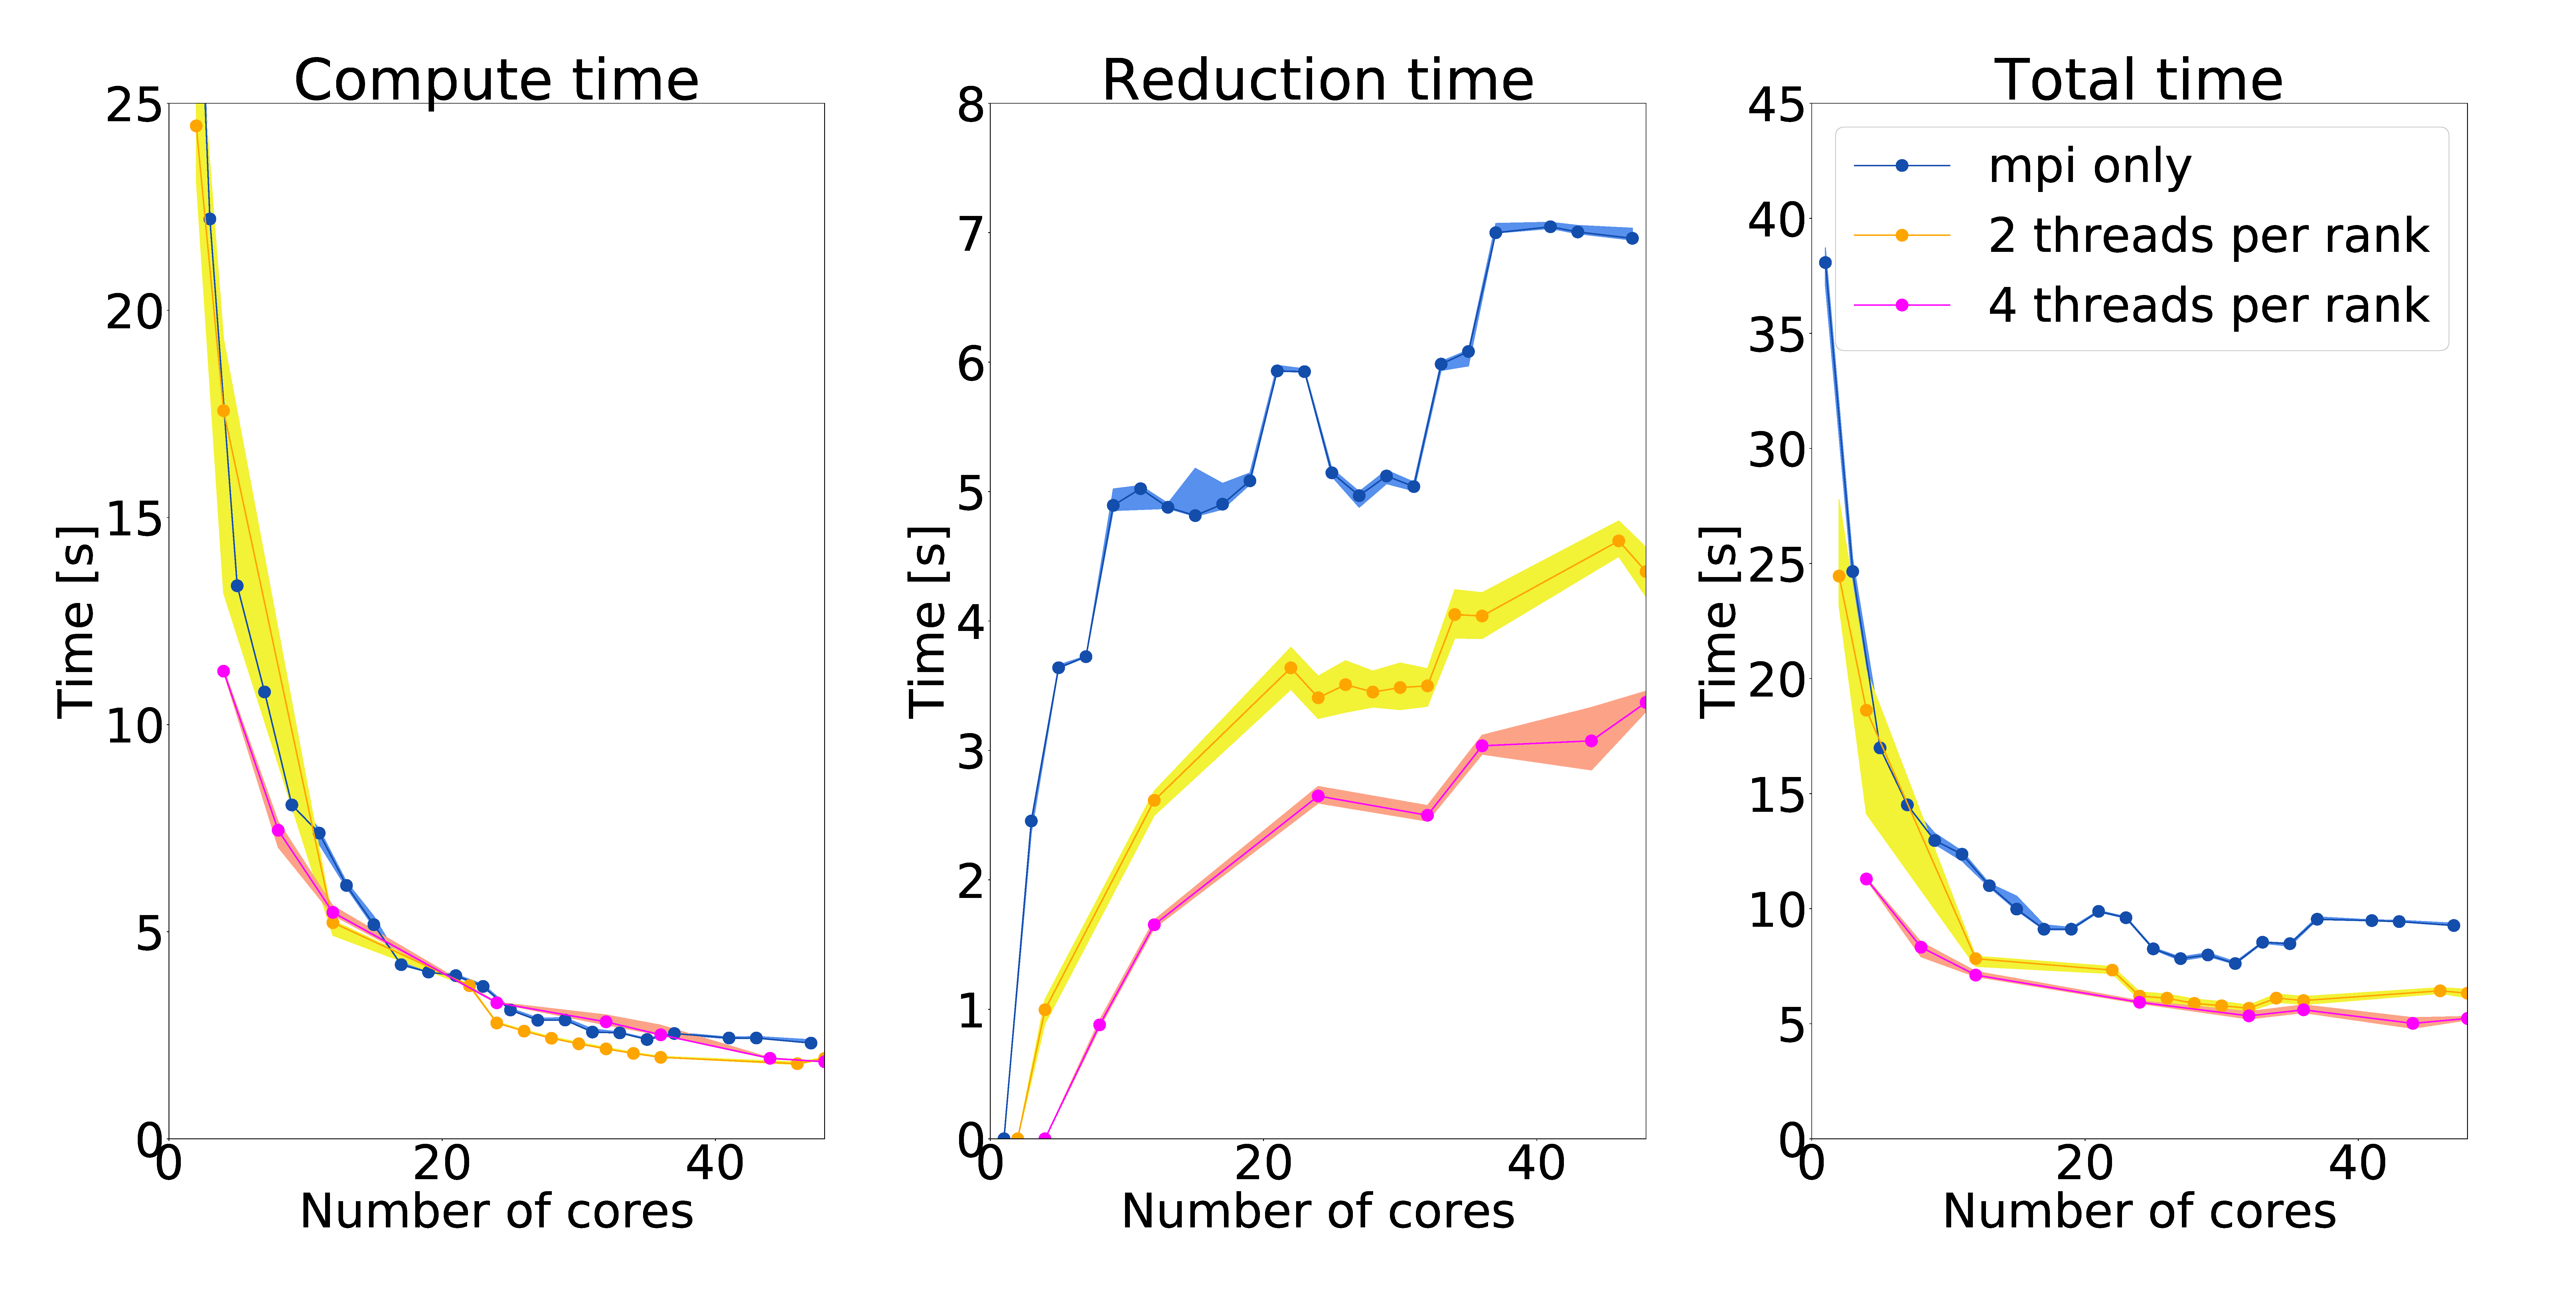
\includegraphics[width=0.5\textwidth]{plots/20000mpi_mixtures_with_everything}
\subcaption{$2\times10^{7}$ vertices}
\caption{Total runtime breakdown on graph with $5\times10^{8}$ edges and $2\times10^{7}$ vertices. The experiment was run on the Euler cluster.}
\label{fig:mixed_euler}
\end{figure}

\autoref{fig:mixed_euler} shows the compute time being largely independent of the mixture. This is a consequence of the graphs sparsity which results in low contention between the OMP threads. The reduction time, however, wildly differs for the different mixtures. For each mixture it increases logarithmically with the number of MPI ranks. This results in the algorithm's performance decreasing as less OMP threads per MPI rank are used.

\mypar{Speedups}

\begin{figure}
\begin{subfigure}[c]{0.23\textwidth}
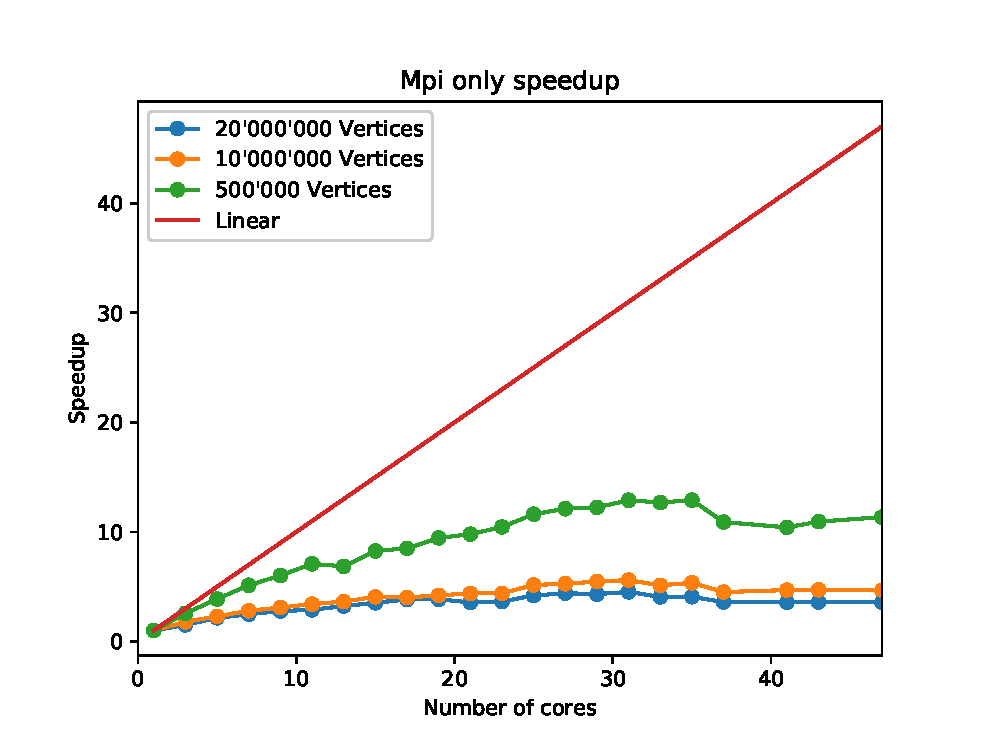
\includegraphics[width=\textwidth]{plots/mpi_speedup_with_ref}
\subcaption{MPI only}
\label{fig:speedup_mpi}
\end{subfigure}
\begin{subfigure}[c]{0.23\textwidth}
\includegraphics[width=\textwidth]{plots/omp_speedup_with_ref}
\subcaption{OMP only}
\label{fig:speedup_omp}
\end{subfigure}
\caption{Speedup of MPI only and OMP only version on three different graphs each with $5\times10^{8}$ edges.}
\label{fig:speedup}
\end{figure}

\autoref{fig:speedup} shows the measured speed up of the MPI only and OMP only version. As one would expect from the results discussed previously the MPI only version achieves better scaling compared to the OMP only version on dense graphs while the OMP only version scales better on sparse graphs.



%Here you evaluate your work using experiments. You start again with a
%very short summary of the section. The typical structure follows.
%
%\mypar{Experimental setup} Specify the platform (processor, frequency, maybe OS, maybe cache sizes)
%as well as the compiler, version, and flags used. If your work is about performance,
%I strongly recommend that you play with optimization flags and consider also icc for additional potential speedup.
%
%Then explain what kind of benchmarks you ran. The idea is to give enough information so the experiments are reproducible by somebody else on his or her code.
%For sorting you would talk about the input sizes. For a tool that performs NUMA optimization, you would specify the programs you ran.

%Next divide the experiments into classes, one paragraph for each. In each class of experiments you typically pursue one questions that then is answered by a suitable plot or plots. For example, first you may want to investigate the performance behavior with changing input size, then how your code compares to external benchmarks.
%
%For some tips on benchmarking including how to create a decent viewgraph see pages 22--27 in \cite{Pueschel:10}.

%{\bf Comments:}
%\begin{itemize}
%\item Create very readable, attractive plots (do 1 column, not 2 column plots
%for this report) with readable font size. However, the font size should also not be too large; typically it is smaller than the text font size.
%An example is in Fig.~\ref{fftperf} (of course you can have a different style).
%\item Every plot answers a question. You state this question and extract the
%answer from the plot in its discussion.
%\item Every plot should be referenced and discussed.
%\end{itemize}

%\begin{figure}\centering
%  \includegraphics[scale=0.33]{dft-performance.eps}
%  \caption{Performance of four single precision implementations of the
%  discrete Fourier transform. The operations count is roughly the
%  same. The labels in this plot are maybe a little bit too small.\label{fftperf}}
%\end{figure}

\section{Conclusions}

The proposed algorithm manages to take advantage of the parallelism available within shared memory units while avoiding excessive communication between them. By choosing the right number of OMP threads per MPI rank the algorithm achieves good scaling across a variety of graphs. The results show our algorithm outperforming the communication-avoiding algorithm \cite{comm_avoiding} in each experiment except for the densest graph on Euler.

%Here you need to summarize what you did and why this is
%important. {\em Do not take the abstract} and put it in the past
%tense. Remember, now the reader has (hopefully) read the report, so it
%is a very different situation from the abstract. Try to highlight
%important results and say the things you really want to get across
%such as high-level statements (e.g., we believe that .... is the right
%approach to .... Even though we only considered x, the
%.... technique should be applicable ....) You can also formulate next
%steps if you want. Be brief. After the conclusions there are only the references.

\section{Future Work}

The main drawback of our algorithm is the reduction step's runtime of $O\left(n \cdot log\left(p\right)\right)$, where $p$ is the number of MPI ranks and $n$ is the number of vertices. For a large number of MPI ranks the $log\left(p\right)$ factor becomes an issue.\\
\replaced[id=R]{Decreasing}{Reducing} the reductions \replaced[id=R]{citical path}{"height"} addresses this problem. In our algorithm this is done by using a mixture of OMP and MPI which reduces the number of MPI ranks. Since OMP does not scale well once the number of OMP threads exceeds the number of cores per CPU this approach is only viable up to a limited number of cores.\\
Another approach would be reducing the work \deleted[id=R]{$n$} done in each reduction step. Due to time constraints we were unable to investigate this approach. One could imagine a more efficient hook tree representation solving this problem.\\
\\
Another drawback of our algorithm is that in order to achieve satisfying performance one needs to find the right mixture of MPI and OMP. While we analysed the behaviour of different mixtures on graphs with varying density we did not come up with an a priori scheme to determine the right mixture. A good heuristic or even a scheme to find the optimal mixture would be worth exploring.

%Here we provide some further tips.

%\mypar{Further general guidelines}
%
%\begin{itemize}
%\item For short papers, to save space, I use paragraph titles instead of
%subsections, as shown in the introduction.
%
%\item It is generally a good idea to break sections into such smaller
%units for readability and since it helps you to (visually) structure the story.
%
%\item The above section titles should be adapted to more precisely
%reflect what you do.
%
%\item Each section should be started with a very
%short summary of what the reader can expect in this section. Nothing
%more awkward as when the story starts and one does not know what the
%direction is or the goal.
%
%\item Make sure you define every acronym you use, no matter how
%convinced you are the reader knows it.
%
%\item Always spell-check before you submit (to us in this case).
%
%\item Be picky. When writing a paper you should always strive for very
%high quality. Many people may read it and the quality makes a big difference.
%In this class, the quality is part of the grade.
%
%\item Books helping you to write better: \cite{Higham:98} and \cite{Strunk:00}.
%
%\item Conversion to pdf (latex users only):
%
%dvips -o conference.ps -t letter -Ppdf -G0 conference.dvi
%
%and then
%
%ps2pdf conference.ps
%\end{itemize}
%
%\mypar{Graphics} For plots that are not images {\em never} generate the bitmap formats
%jpeg, gif, bmp, tif. Use eps, which means encapsulate postscript. It is
%scalable since it is a vector graphic description of your graph. E.g.,
%from Matlab, you can export to eps.
%
%The format pdf is also fine for plots (you need pdflatex then), but only if the plot was never before in the format
%jpeg, gif, bmp, tif.


% References should be produced using the bibtex program from suitable
% BiBTeX files (here: bibl_conf). The IEEEbib.bst bibliography
% style file from IEEE produces unsorted bibliography list.
% -------------------------------------------------------------------------
\bibliographystyle{IEEEbib}
\bibliography{bibl_conf}

\end{document}

